\documentclass[11pt,a4paper]{article}
\usepackage[T1]{fontenc}\usepackage{charter}\usepackage[scaled=0.92]{helvet}\usepackage{courier}\usepackage{xurl}
\usepackage[utf8]{inputenc}
\usepackage[margin=2.4cm]{geometry}
\usepackage{microtype,booktabs,tabularx,array,enumitem,xcolor,graphicx,float,caption}
\usepackage[most]{tcolorbox}
\usepackage{listings}
\usepackage{titlesec}
\usepackage{tikz}
\usetikzlibrary{arrows.meta,positioning}
\usepackage[hidelinks]{hyperref}

\definecolor{accent}{HTML}{C74634}
\definecolor{ink}{HTML}{2B2B2B}
\definecolor{codebg}{HTML}{F5F5F2}
\definecolor{notebg}{HTML}{EEF3F8}
\definecolor{noteframe}{HTML}{4A6C8F}
\definecolor{warnbg}{HTML}{FBF1EE}
\definecolor{okgreen}{HTML}{4E8A3E}
\definecolor{errblue}{HTML}{4A7FB5}

\color{ink}
\titleformat{\section}{\sffamily\Large\bfseries\color{accent}}{\thesection}{0.6em}{}
\titleformat{\subsection}{\sffamily\large\bfseries}{\thesubsection}{0.6em}{}
\titleformat{\subsubsection}{\sffamily\normalsize\bfseries}{}{0em}{}
\titlespacing*{\section}{0pt}{1.6em}{0.6em}
\setlength{\parskip}{0.45em}
\setlength{\parindent}{0pt}
\setlist{itemsep=0.15em,topsep=0.3em}
\captionsetup{font={small,sf},labelfont=bf}

\lstdefinestyle{sql}{
  language=SQL, basicstyle=\ttfamily\small, keywordstyle=\bfseries\color{accent},
  commentstyle=\itshape\color{gray}, stringstyle=\color{okgreen!70!black},
  backgroundcolor=\color{codebg}, frame=single, rulecolor=\color{codebg},
  framesep=6pt, xleftmargin=6pt, xrightmargin=6pt, breaklines=true,
  columns=fullflexible, keepspaces=true, showstringspaces=false,
  morekeywords={BEGIN,END,DECLARE,TABLE,RETURN}}
\lstset{style=sql}

\newtcolorbox{note}[1][Note]{enhanced,colback=notebg,colframe=noteframe,boxrule=0pt,leftrule=3pt,arc=0pt,
  fonttitle=\sffamily\bfseries\small,coltitle=noteframe,colbacktitle=notebg,title=#1,attach title to upper={\par},left=8pt,right=8pt,top=6pt,bottom=6pt}
\newtcolorbox{warn}[1][Caution]{enhanced,colback=warnbg,colframe=accent,boxrule=0pt,leftrule=3pt,arc=0pt,
  fonttitle=\sffamily\bfseries\small,coltitle=accent,colbacktitle=warnbg,title=#1,attach title to upper={\par},left=8pt,right=8pt,top=6pt,bottom=6pt}

\newcolumntype{L}{>{\raggedright\arraybackslash}X}
\renewcommand{\arraystretch}{1.25}

\emergencystretch=3em
\begin{document}

\begin{titlepage}
\vspace*{4cm}
{\sffamily\color{accent}\rule{2.5cm}{3pt}\par}
\vspace{0.8em}
{\sffamily\fontsize{30}{36}\selectfont\bfseries Workflows in\\[0.2em] Oracle APEX\par}
\vspace{1em}
{\sffamily\Large A practical guide to tasks, workflows and their APIs\par}
\vspace{3cm}
\begin{tcolorbox}[enhanced,colback=codebg,colframe=codebg,arc=0pt,left=10pt,right=10pt,top=8pt,bottom=8pt]
\small\textbf{\sffamily Disclaimer.} This guide is based on practical experience and publicly available sources. It is a simplified reference, not an exhaustive or authoritative one. Details may be inaccurate or outdated, and behaviour can vary with the APEX version, configuration or environment. Always verify against the official Oracle documentation and test in a non-production environment before relying on any of it. Written for APEX 23.2--24.2.
\end{tcolorbox}
\vfill
\end{titlepage}

\tableofcontents
\newpage

\section{What Is a Workflow in APEX?}
A workflow in APEX is a structured process that automates business rules, approvals and sequences of tasks. It can combine automated steps (PL/SQL, REST calls, e-mails) with human steps (approvals and actions performed by users).

Every workflow instance is started for one business record, identified by its \textbf{detail primary key} (\texttt{detail\_pk}). This key is passed in when the workflow starts, carried through every activity and task, and can be referenced at any point to retrieve the record's data.

\section{Tasks}
\subsection{What a Task Is}
Tasks are the \emph{human} steps of a workflow: steps that require someone to act before the workflow can continue.

\textit{Example.} When a purchase request is submitted, it is sent to a reviewer who must approve or reject it. This is an approval task; its outcome decides whether the request moves on to the next approver or is closed.

\subsection{Task Definitions}
Tasks are defined in \textbf{Shared Components $\rightarrow$ Task Definitions}. There are two types:
\begin{itemize}
\item \textbf{Approval task:} the user approves or rejects. The outcome is stored in a workflow variable, typically read by a \emph{Switch} activity to send the workflow down the right branch.
\item \textbf{Action task:} the user simply completes the task (marks it as done). There is no approve/reject outcome.
\end{itemize}

\subsection{Task Definition Actions}
Task definition actions run automatically when something happens to a task. They can send an e-mail, send a push notification, or execute PL/SQL code. Unlike workflow activities, they run \emph{inside the task context} and are tied to task events:

\begin{center}\small
\begin{tabular}{@{}lll@{}}
\toprule
\multicolumn{3}{@{}l}{\sffamily\bfseries Task events} \\
\midrule
Create & Complete & Claim \\
Cancel & Release & Delegate \\
Update Comment & Update Priority & Update Parameter \\
Request Information & Submit Information & Before Expire, Expire \\
\bottomrule
\end{tabular}
\end{center}

\begin{note}[Task action or workflow activity?]
Use a task definition action when you need task-specific data, for example an e-mail that includes task parameters, or an update based on what the user entered in the task. If no task data is needed, a normal workflow activity is usually simpler.
\end{note}

\subsection{Task Details Page}
Each task has a \textbf{Task Details page}, which APEX can generate for you. It shows the data of one task instance and can differ from what is shown in the Unified Task List.
\begin{itemize}
\item The bind variable \texttt{:APEX\$TASK\_PK} holds the detail primary key of the task and can be used to query the related business record.
\item What is displayed (subject, details) comes from the task definition's \emph{Action Source}.
\item The page can be customised freely, and its actions can be implemented with the \texttt{APEX\_HUMAN\_TASK} package.
\end{itemize}

\textit{Example:} show the order number in the task subtitle by querying the record behind the task.
\begin{lstlisting}
select order_id
  from orders
 where order_id = :APEX$TASK_PK;
\end{lstlisting}

A task can also have a deadline (due date) after which it expires.

\subsection{Participants and Roles}
Task participants define who can act on a task. They are of type \emph{Potential Owner} or \emph{Business Administrator}, and the task appears in their Unified Task List.
\begin{itemize}
\item \textbf{Potential owner:} can claim an unassigned task and thereby become its actual owner. A task can have several potential owners.
\item \textbf{Actual owner:} works on a claimed task and can approve, reject or complete it.
\item \textbf{Initiator:} the user who started the task. Can change its priority and cancel it (if enabled).
\item \textbf{Business administrator:} oversees all tasks of a task definition; can delegate them, change their priority and add potential owners (if enabled).
\end{itemize}

\begin{table}[H]
\centering\small
\begin{tabularx}{\textwidth}{@{}l>{\centering\arraybackslash}p{1.6cm}LL>{\centering\arraybackslash}p{2.2cm}@{}}
\toprule
\sffamily\bfseries Action & \sffamily\bfseries Initiator & \sffamily\bfseries Potential owner & \sffamily\bfseries Actual owner & \sffamily\bfseries Business admin \\
\midrule
Claim & -- & Yes, if the task is unassigned & -- & -- \\
Complete (approve / reject) & -- & Yes, from the task list, or by claiming it on the details page & Yes, from the task list or the details page & -- \\
Delegate & -- & -- & Yes & Yes \\
Release & -- & -- & Yes & -- \\
Cancel (if enabled) & Yes & -- & -- & -- \\
Add potential owner (if enabled) & -- & -- & -- & Yes \\
Add comment & Yes & Yes & Yes & Yes \\
Set priority & Yes & -- & -- & Yes \\
\bottomrule
\end{tabularx}
\caption{Task actions by role.}
\end{table}

\begin{note}[Good to know]
\begin{itemize}[leftmargin=1.2em]
\item A task with a single potential owner is assigned to that user directly; with several potential owners it stays unassigned until someone claims it.
\item An actual owner can delegate a task to another user, typically someone with the same role.
\item Every task and workflow instance is stored by APEX and can be queried through views (Section~\ref{sec:views}).
\item All task actions are available on the Task Details page, and each one also exists as a procedure or function in \texttt{APEX\_HUMAN\_TASK}, so it can be called from automations or other code.
\end{itemize}
\end{note}

\subsection{Task States}
Figure~\ref{fig:taskstates} and Table~\ref{tab:taskstates} show the life cycle of a task.

\begin{figure}[H]
\centering
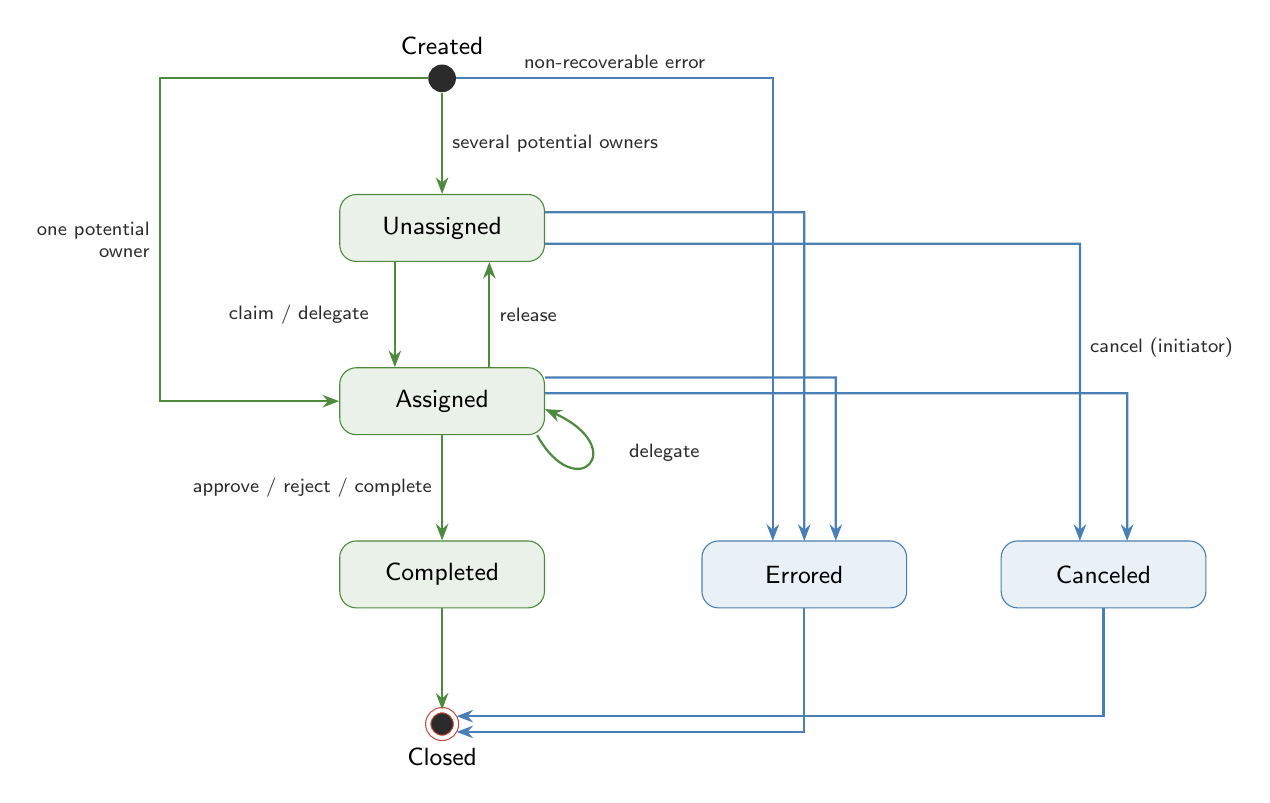
\begin{tikzpicture}[
  font=\sffamily\small,
  st/.style={draw=okgreen,fill=okgreen!12,rounded corners=6pt,minimum width=2.6cm,minimum height=0.85cm},
  ex/.style={draw=errblue,fill=errblue!12,rounded corners=6pt,minimum width=2.6cm,minimum height=0.85cm},
  dot/.style={circle,fill=ink,minimum size=10pt,inner sep=0},
  ok/.style={-{Stealth[length=6pt]},okgreen,thick},
  bad/.style={-{Stealth[length=6pt]},errblue,thick},
  lab/.style={font=\sffamily\scriptsize,text=ink}]
\node[dot,label=above:{Created}] (start) at (0,0) {};
\node[st] (un) at (0,-1.9) {Unassigned};
\node[st] (as) at (0,-4.1) {Assigned};
\node[st] (co) at (0,-6.3) {Completed};
\node[ex] (er) at (4.6,-6.3) {Errored};
\node[ex] (ca) at (8.4,-6.3) {Canceled};
\node[dot,draw=accent,double,double distance=1.5pt,label=below:{Closed}] (end) at (0,-8.2) {};

\draw[ok] (start) -- node[lab,right]{several potential owners} (un);
\draw[ok] (start.west) -- ++(-3.4,0) |- node[lab,pos=0.25,left,align=right]{one potential\\owner} (as.west);
\draw[ok] ([xshift=-6mm]un.south) -- node[lab,left,xshift=-2mm]{claim / delegate} ([xshift=-6mm]as.north);
\draw[ok] ([xshift=6mm]as.north) -- node[lab,right]{release} ([xshift=6mm]un.south);
\draw[ok] ([xshift=-1mm]as.south east) .. controls +(0.5,-0.9) and +(1.1,-0.5) .. ([yshift=-1mm]as.east);
\node[lab,anchor=west] at (2.25,-4.75) {delegate};
\draw[ok] (as) -- node[lab,left]{approve / reject / complete} (co);
\draw[ok] (co) -- (end);

\draw[bad] (start.east) -- node[lab,above]{non-recoverable error} (4.2,0) -- (4.2,-5.875);
\draw[bad] ([yshift=2mm]un.east) -- (4.6,-1.7) -- (4.6,-5.875);
\draw[bad] ([yshift=-2mm]un.east) -- (8.1,-2.1) -- node[lab,right,pos=0.35]{cancel (initiator)} (8.1,-5.875);
\draw[bad] ([yshift=3mm]as.east) -- (5.0,-3.8) -- (5.0,-5.875);
\draw[bad] ([yshift=1mm]as.east) -- (8.7,-4.0) -- (8.7,-5.875);
\draw[bad] (er.south) |- ([yshift=-1mm]end.east);
\draw[bad] (ca.south) |- ([yshift=1mm]end.east);
\end{tikzpicture}
\caption{Task states and transitions. Green: normal flow; blue: exceptions.}
\label{fig:taskstates}
\end{figure}

\begin{table}[H]
\centering\small
\begin{tabularx}{\textwidth}{@{}llL@{}}
\toprule
\sffamily\bfseries State & \sffamily\bfseries Stage / category & \sffamily\bfseries Possible transitions \\
\midrule
Created & Initial / normal & \textbf{Unassigned} if there are several potential owners; \textbf{Assigned} if there is one; \textbf{Errored} on a non-recoverable error. \\
Unassigned & Intermediate / normal & \textbf{Assigned} when a user claims it or it is delegated; \textbf{Errored}; \textbf{Canceled} by the initiator. \\
Assigned & Intermediate / normal & \textbf{Completed} when the owner approves, rejects or completes it; \textbf{Unassigned} when the owner releases it; \textbf{Assigned} (new owner) when delegated; \textbf{Errored}; \textbf{Canceled} by the initiator. \\
Completed & Final / normal & None. \\
Errored & Final / exception & None. \\
Canceled & Final / user interrupted & None. \\
\bottomrule
\end{tabularx}
\caption{Task states and transitions.}
\label{tab:taskstates}
\end{table}

\subsection{Unified Task List}
The Unified Task List works like an inbox for tasks. Its exact name and layout depend on your application, but it offers three report contexts:
\begin{itemize}
\item \textbf{My Tasks:} tasks where you are a potential or actual owner. You can approve, reject or complete them.
\item \textbf{Admin Tasks:} tasks where you are business administrator. You can change their priority or delegate them.
\item \textbf{Initiated by Me:} tasks you started. You can change their priority or cancel them.
\end{itemize}
Each task is shown with its subject and initiator. Clicking a task opens its Task Details page, which can be customised to show what the user needs. The generated page includes buttons for the standard actions; if some do not fit your process, re-implement them with the \texttt{APEX\_HUMAN\_TASK} package.

\begin{warn}[Deprecated package]
\texttt{APEX\_APPROVAL} is deprecated and will be removed in a future release. Use \texttt{APEX\_HUMAN\_TASK} instead; it offers the same procedures and functions.
\end{warn}

\subsection{Task Parameters}
Task parameters are declared in the task definition. They are used to determine potential owners, to display information, or inside task action code. Their values are set when the workflow creates the task, and they can be updated later (for example from the Task Details page) and read back from another activity.

\subsection{Comments}
Comments are shared between everyone involved in a task. They are typically used to discuss a request before claiming it or to explain a delegation.

\subsection{Task Visibility Pitfalls}
\begin{itemize}
\item If an approval task does not allow the initiator to approve it, the task does not appear for the initiator, even if they are listed as a potential owner.
\item Potential owners are evaluated when the task is created. A user given the required role \emph{afterwards} will not see the existing task. Make sure roles are assigned before the workflow instance starts.
\item If the workflow has already started, retrying the task (or canceling and recreating it) re-evaluates the potential owners and includes the new users.
\end{itemize}

\section{Working with the APIs}
\label{sec:views}
\subsection{Useful Views}
\begin{center}\small
\begin{tabularx}{0.9\textwidth}{@{}lL@{}}
\toprule
\sffamily\bfseries View & \sffamily\bfseries Content \\
\midrule
\texttt{APEX\_WORKFLOWS} & All workflow instances, with their state and \texttt{detail\_pk}. \\
\texttt{APEX\_WORKFLOW\_VARIABLES} & Current values of workflow variables. \\
\texttt{APEX\_TASKS} & Human task instances (task ID, state, \texttt{detail\_pk}, \dots). \\
\texttt{APEX\_TASK\_PARAMETERS} & Parameter values of each task. \\
\bottomrule
\end{tabularx}
\end{center}

\subsection{Reading Tasks}
Display the details of one task, for example in a Classic Report on the Task Details page:
\begin{lstlisting}
select *
  from table ( apex_human_task.get_tasks (
                 p_context            => 'SINGLE_TASK',
                 p_task_id            => :P1_TASK_ID,
                 p_show_expired_tasks => 'N' ) );
\end{lstlisting}
If a Human Task activity stores the task ID in a workflow variable, that ID can be used later in the workflow to read the task's state or parameters.

\subsection{Completing a Task from Code}
Tasks are normally completed by users, but they can also be completed programmatically, for example when a condition is met:
\begin{lstlisting}
begin
  apex_human_task.complete_task (
    p_task_id => :TASK_ID,
    p_outcome => apex_human_task.c_task_outcome_approved );
end;
\end{lstlisting}
Always change tasks through the API rather than updating tables directly: the views are read-only, and the API keeps the workflow engine consistent.

\subsection{Passing Data Between Tasks}
\textit{Problem:} Task 2 needs a value (for example a user name) that was entered in Task 1.

\textit{Approach:}
\begin{enumerate}
\item In Task 1, store the value in a task parameter (for example by updating it from the Task Details page).
\item Store Task 1's ID in a workflow variable, e.g.\ \texttt{TASK1\_ID}.
\item Between the two tasks, add an \emph{Execute Code} or \emph{Invoke API} activity that reads the parameter:
\begin{lstlisting}
:TASK1_USER := apex_human_task.get_task_parameter_value (
                 p_task_id         => :TASK1_ID,
                 p_param_static_id => 'USER_NAME' );
\end{lstlisting}
\item Store the result in another workflow variable (here \texttt{TASK1\_USER}).
\item In Task 2, use \texttt{TASK1\_USER} in a parameter, in the subject, or to assign the task.
\end{enumerate}

\section{Workflows}
\subsection{How a Workflow Runs}
A workflow follows its diagram. It moves from activity to activity according to task outcomes and workflow variables, running procedures, updating data and recording every step as it goes. Each human task it creates appears in the Unified Task List, and every user action (approve, reject, complete) is recorded by the workflow engine for auditing.

A workflow has a single \emph{Start} activity and is started with a detail primary key. From then on, its details, transitions and states are logged and visible in the Workflow Console. Each activity stays active until it finishes: a human task until it is approved, rejected or completed, an automated activity until its code has run. The engine then moves to the next activity.

The \texttt{detail\_pk} is propagated to every task and stored with it (see \texttt{APEX\_TASKS}). It is what links all the data of one process together.

\textit{Example.} In an expense-report process, the report ID groups all the expense lines submitted together. Passing that ID as the detail primary key lets every activity retrieve the full report (status, employee, lines, totals) without extra lookups.

\begin{lstlisting}
-- details of one workflow instance
select *
  from table ( apex_workflow.get_workflows (
                 p_context     => 'SINGLE_WORKFLOW',
                 p_workflow_id => :P1_WORKFLOW_ID ) );

-- business records whose workflow was terminated
select detail_pk
  from apex_workflows
 where state_code = 'TERMINATED';
\end{lstlisting}

\subsection{Workflow States}
Workflow state transitions are made by the engine, through the API, or as the result of a user action; for example, a workflow moves from \emph{Active} to \emph{Completed} after a final approval.

\begin{table}[H]
\centering\small
\begin{tabularx}{\textwidth}{@{}llL@{}}
\toprule
\sffamily\bfseries State & \sffamily\bfseries Category & \sffamily\bfseries Possible transitions \\
\midrule
Active & Normal & \textbf{Completed} when an end activity is reached. \textbf{Faulted} when the instance cannot be created (invalid parameters, no start activity or more than one) or an activity fails. \textbf{Suspended} by API or user request. \textbf{Terminated} by API or user request, or when an end activity set to terminate is reached. \\
Completed & Normal & None. \\
Faulted & Exception & \textbf{Active} when retried successfully. \textbf{Suspended} or \textbf{Terminated} by API or user request. A faulted workflow can be retried after its variables are fixed, or terminated if it should not run any more. \\
Suspended & Normal & \textbf{Active} when resumed. \textbf{Faulted} when an outstanding asynchronous activity returns an error. \textbf{Terminated} by API or user request. A workflow resumes at its current activity by default; \texttt{APEX\_WORKFLOW.RESUME} can resume it at any activity (24.2). \\
Terminated & Exception & None. A terminated instance cannot be retried. \\
\bottomrule
\end{tabularx}
\caption{Workflow states and transitions.}
\end{table}

\subsection{Activity States}
An activity is always in exactly one state:
\begin{table}[H]
\centering\small
\begin{tabularx}{\textwidth}{@{}llL@{}}
\toprule
\sffamily\bfseries State & \sffamily\bfseries Category & \sffamily\bfseries Possible transitions \\
\midrule
Active & Normal & \textbf{Completed} when it succeeds and the workflow continues. \textbf{Faulted} when it, or something leading into or out of it, fails. \textbf{Terminated} when the workflow is terminated. \textbf{Waiting} when it waits for a result, e.g.\ an approval or an asynchronous call. \\
Waiting & Normal & \textbf{Active} when the awaited operation finishes (this can be so quick that users never see the waiting state). \textbf{Faulted} if processing fails. \textbf{Terminated} if the workflow is terminated. \\
Completed & Normal & None. \\
Faulted & Exception & \textbf{Active} when the workflow is retried: the engine runs the activity again. \\
Terminated & Exception & None. \\
\bottomrule
\end{tabularx}
\caption{Activity states and transitions.}
\end{table}

\subsection{Parameters and Variables}
\textbf{Workflow parameters} are the inputs passed to a workflow when an instance starts; for a laptop-request approval, these could be the employee ID and the laptop type. They support data types and format masks and can be based on SQL queries or page items. Parameters have a direction:
\begin{itemize}
\item \textbf{In:} read-only inside the workflow.
\item \textbf{Out} and \textbf{In/Out:} can be updated while the instance runs. They can only be based on workflow items (variables and parameters), and \emph{Out} values can only be returned when the workflow is invoked from another workflow, not from a page process.
\end{itemize}

\textbf{Workflow variables} belong to a workflow version and can change at runtime. They support data types and format masks, can be initialised from SQL queries, expressions, function bodies or parameters, and may start as \texttt{NULL}. A variable is updated by:
\begin{itemize}
\item the result of a completed activity (for example a task outcome);
\item a call to \texttt{apex\_workflow.update\_variables};
\item an administrator editing it in the workflow details page.
\end{itemize}

\subsection{Development and Active Versions}
A new workflow version starts in \textbf{development} mode, where it can be changed freely. Do all testing in this mode.

When the application is ready, the version must be \textbf{activated}. An active version can only be started when the application itself is not in development mode, and some of its features can no longer be edited or added.

Activating a new version makes the previous one obsolete, but instances already started keep running with the version they were created with. Workflow instances of an active version cannot be deleted: deactivate the version first, then remove its instances.

\section{Troubleshooting}
\subsection{Error ORA-20987 When a Task Is Created}
\begin{lstlisting}[language={},keywordstyle=]
ORA-20987: APEX - The creation of a new Task for Task Definition <id>
in application <app_id> failed. SQLCODE: -20001
\end{lstlisting}
Likely causes:
\begin{itemize}
\item The task definition's SQL query (Action Source) is invalid or returns nothing. Fix it, or set the source to \emph{None} if it is not needed.
\item A task definition action that runs \emph{on Create} raised an unhandled error. Check every action attached to the event at which the error appears.
\end{itemize}

\subsection{Rolling Back Changes After a Workflow Is Terminated}
When a workflow is terminated part-way, the changes its activities already made to the database stay in place. Two strategies help:
\begin{itemize}
\item \textbf{Revert on termination.} Run logic when a workflow is terminated that resets every value it changed. This works, but becomes slow and fragile if the workflow made many changes.
\item \textbf{Write at the end.} Keep intermediate values in workflow variables and write them to the database only when the workflow completes. This is cleaner, but harder to manage in complex workflows.
\end{itemize}
\textit{Example.} A workflow sets a record's status to ``In review'' when it starts, then creates a human task; when the task is completed, it sets the final status. If the workflow is terminated in between, an \textbf{automation} that looks for terminated workflows can set the status back and cancel the pending task:
\begin{lstlisting}
select w.detail_pk
  from apex_workflows w
 where w.state_code = 'TERMINATED'
   and w.end_time   > apex_automation.get_last_run;
\end{lstlisting}

\subsection{The Automation Does Not Run}
\begin{itemize}
\item Check that the workflow's \texttt{state\_code} really becomes \texttt{TERMINATED}.
\item Temporarily remove the \texttt{end\_time > apex\_automation.get\_last\_run} filter and run it again.
\item Check that \texttt{detail\_pk} actually contains the expected record ID; if it is empty, the workflow was started without a detail primary key.
\item Check that none of the columns used in the automation's conditions are \texttt{NULL}.
\end{itemize}

\subsection{A User Cannot See a Task}
\begin{itemize}
\item The user was created, or given the required role, after the task was created (see \emph{Task Visibility Pitfalls}).
\item Fix: retry the task, or have the initiator cancel it and start it again, so that potential owners are re-evaluated.
\item To prevent it: assign roles before starting workflows, or add an automation that notifies the business administrator when a new user is added.
\end{itemize}

\section{References}
\begin{itemize}
\item Oracle, \emph{Managing Workflows and Tasks} (APEX 24.1 App Builder guide): \url{https://docs.oracle.com/en/database/oracle/apex/24.1/htmdb/managing-workflows-and-tasks.html}
\item Oracle, \emph{APEX\_HUMAN\_TASK} package reference: \url{https://docs.oracle.com/en/database/oracle/apex/23.2/aeapi/APEX_HUMAN_TASK.html}
\item Oracle, \emph{APEX\_WORKFLOW} package reference: \url{https://docs.oracle.com/en/database/oracle/apex/24.1/aeapi/APEX_WORKFLOW.html}
\item Oracle, \emph{Example workflows} (Sample Workflow, Approvals and Tasks app, available from the gallery under App Builder $\rightarrow$ Create): \url{https://docs.oracle.com/en/database/oracle/apex/24.1/htmdb/example-workflows.html}
\item Oracle LiveLabs workshop on APEX workflows: \url{https://apexapps.oracle.com/pls/apex/r/dbpm/livelabs/run-workshop?p210_wid=3880}
\item A.~Chatterjee, tutorials on the Oracle APEX blog: \url{https://blogs.oracle.com/authors/ananya-chatterjee}
\item P.~Hartenfeller, \emph{APEX 23.2 Workflows: first look}: \url{https://hartenfeller.dev/blog/apex-23-2-workflows-first-look}
\item Novoshore, \emph{Business processes with APEX 24.2 workflows}: \url{https://www.novoshore.com/2025/02/24/business-processes-with-apex-24-2-workflows-a-practical-demo/}
\item \emph{Handling terminations in Oracle APEX workflow}: \url{https://ebs-apex.hashnode.dev/handling-terminations-in-oracle-apex-workflow}
\item Oracle APEX blog, \emph{New in APEX 24.2: workflow within workflow, out parameters, copy and more}: \url{https://blogs.oracle.com/apex/post/new-in-apex-242-workflow-within-workflow-out-parameters-copy-and-more}
\item Oracle APEX blog, \emph{APEX 24.2: resume workflows from any activity}: \url{https://blogs.oracle.com/apex/post/apex-242-resume-workflows-from-any-activity}
\item Oracle forums, \emph{Updating workflow variable from task}: \url{https://forums.oracle.com/ords/apexds/post/updating-workflow-variable-from-task-6284}
\end{itemize}

\end{document}
